\textbf{Authors: \\}
\citefirstlastauthor{paper_a}

\textbf{Published as: \\}
\fullcite{paper_a}

\textbf{Abstract: \\}
\citefield{paper_a}{abstract}

\textbf{Keywords: \\}
\citefield{paper_a}{keywords}

\clearpage

\begin{refsection}

\section{Introduction}
\label{a:sec:introduction}

\Ac{pm} is a collection of data-driven techniques that aim to provide analytical support for \ac{bpm} using process execution data from event logs \citep{Dumas.2018}. 

\Cref{a:fig:giraffe} shows a giraffe.

\begin{figure}
    \centering
    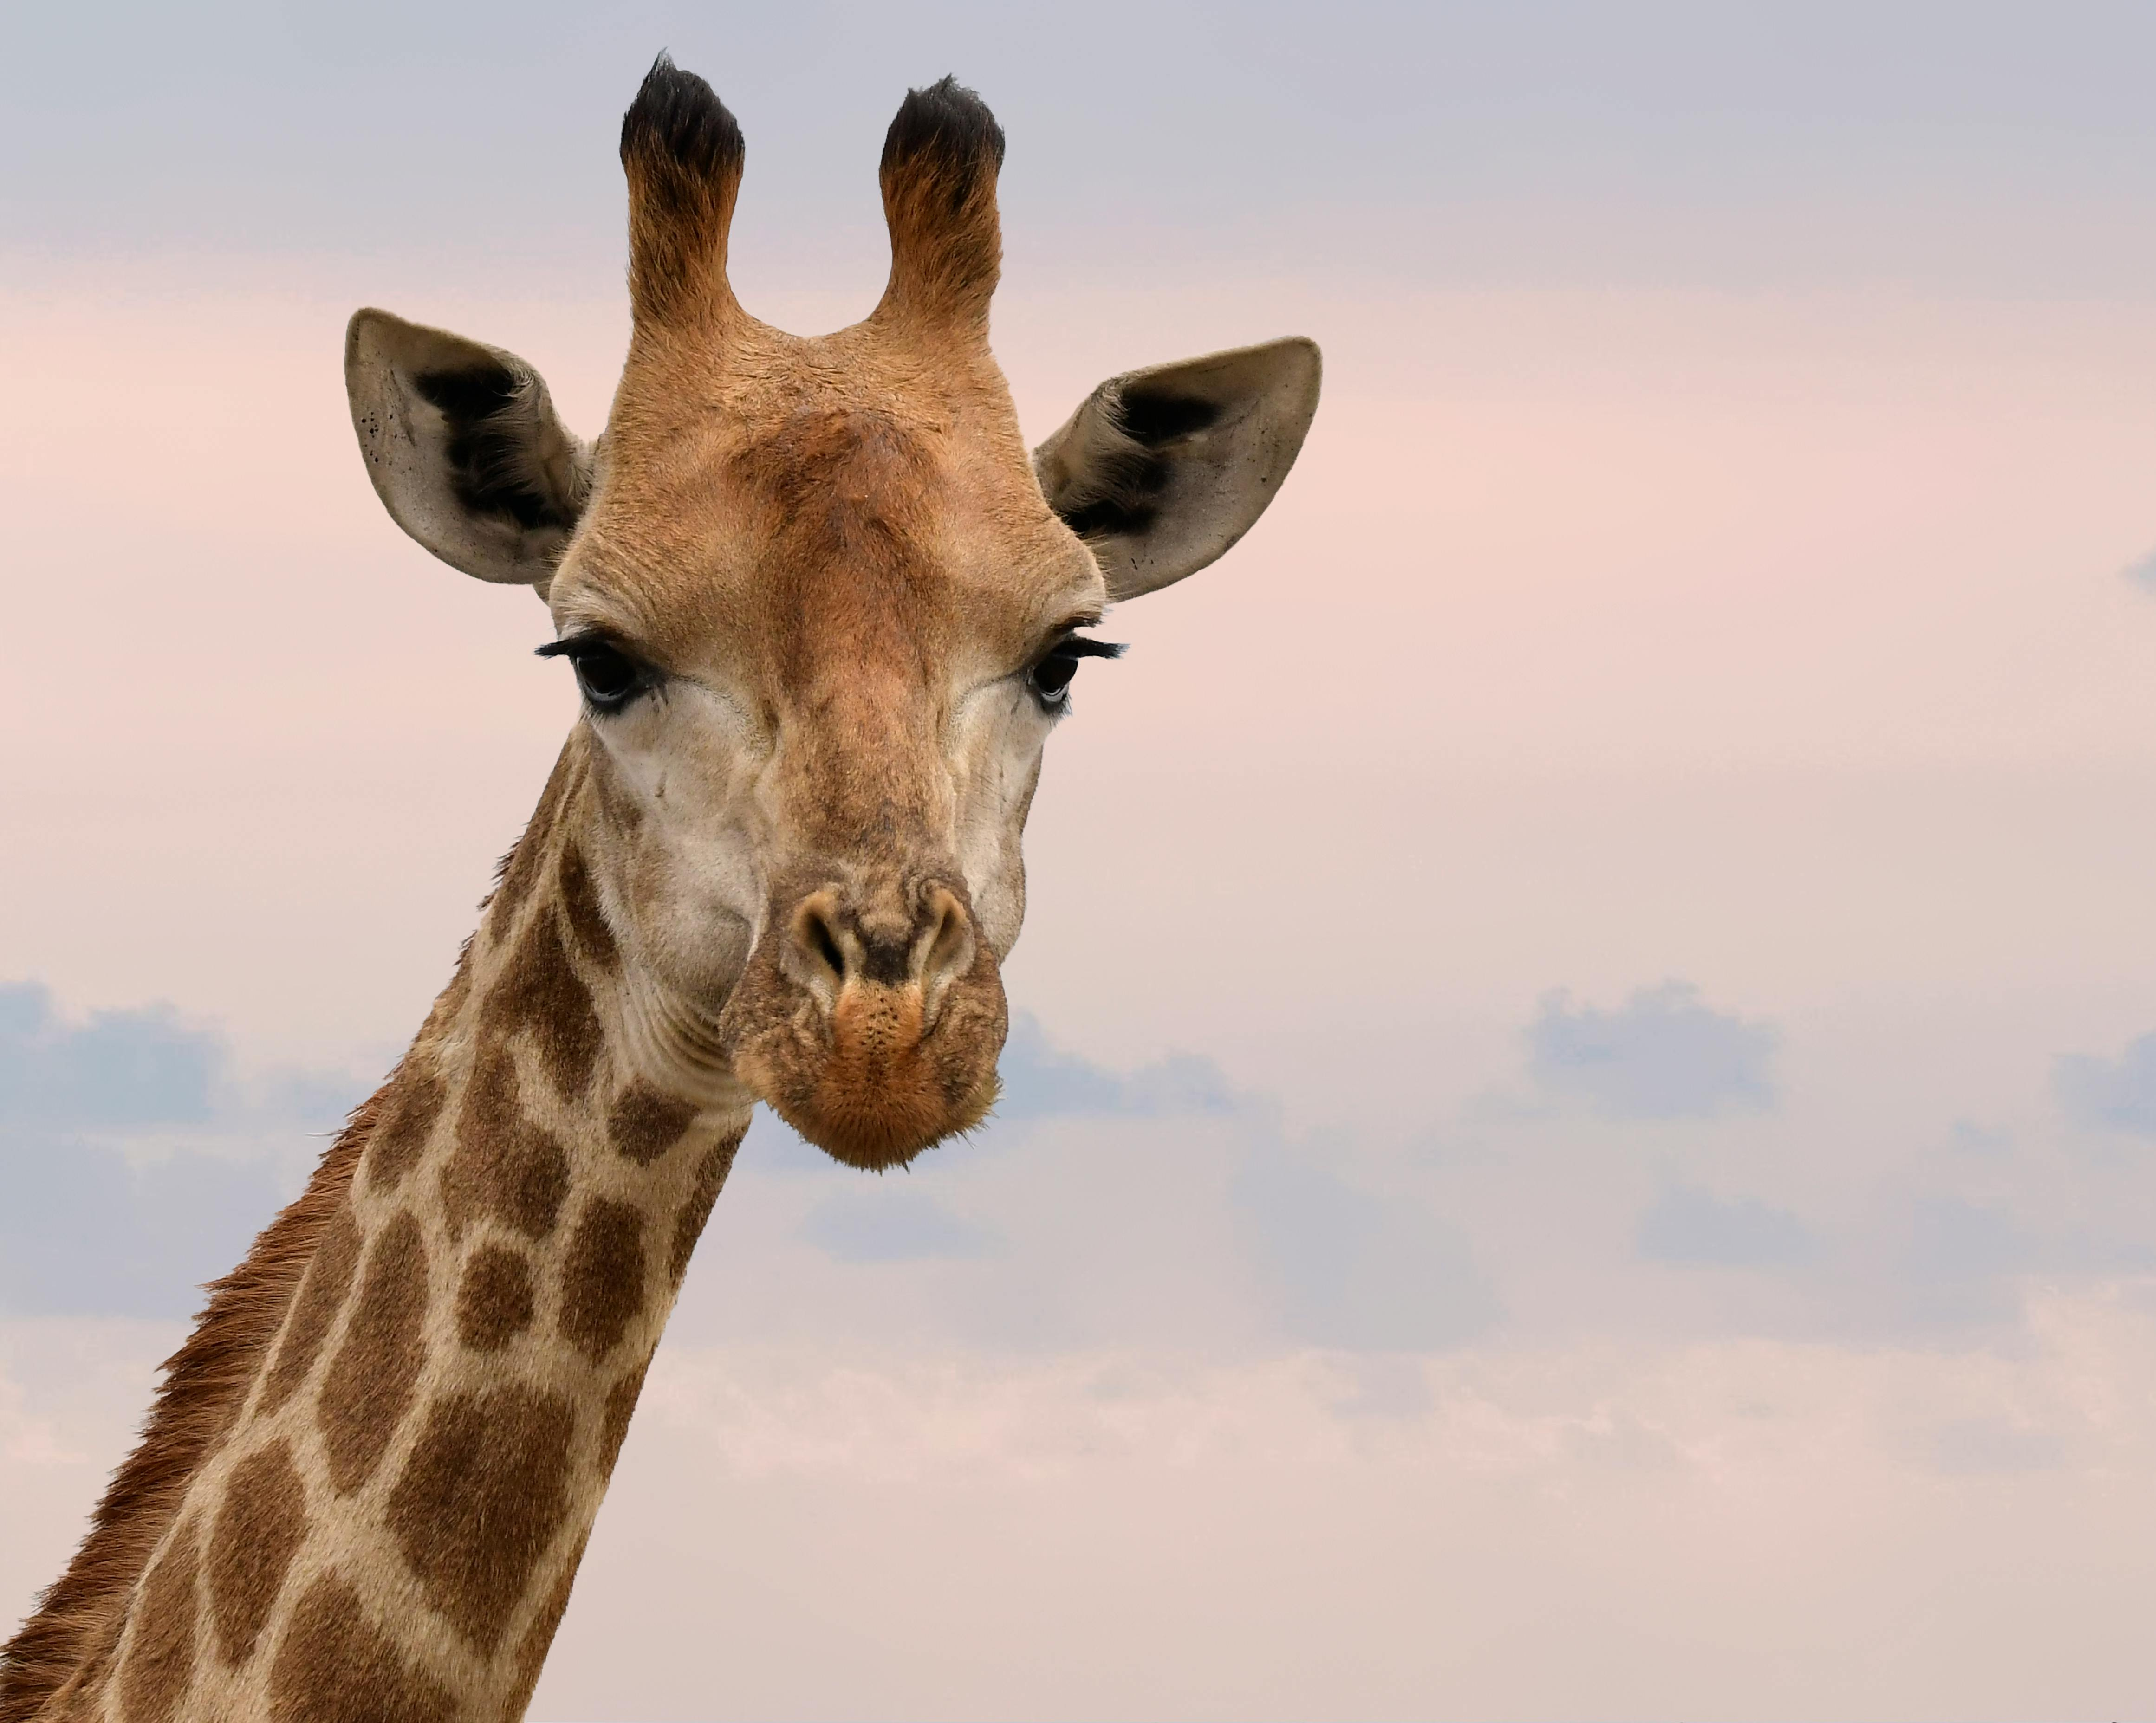
\includegraphics[width=0.5\linewidth]{figures/paper_a/pexels-frans-van-heerden-201846-802112.jpg}
    \caption{Giraffe, Frans van Heerden: https://www.pexels.com/de-de/foto/nahaufnahme-fotografie-der-giraffe-802112/ }
    \label{a:fig:giraffe}
\end{figure}

\section*{References}
\printbibliography[heading=none]
\end{refsection}